\documentclass{article}

\usepackage{graphicx}
\usepackage{tikz}
\usepackage{multirow}
%\documentclass{article}
\usetikzlibrary{positioning}
\usetikzlibrary{3d} % Para trabajar con proyecciones 3D
%\usetikzlibrary{tikz-3dplot}
%\usepackage[spanish]{babel}
\usetikzlibrary{shapes.misc, arrows, positioning}
\usepackage{float}
\usepackage{amsmath}
\usepackage{tikz-3dplot}
\usepackage{pgfplots}
\usepackage{wrapfig}
\usepackage{verbatim}
\usepackage{empheq}
\pgfplotsset{compat=1.18}


\begin{document}
   
\title{\LARGE Medios de Enlace: Una guía por el electromagnetismo \\ 
{\small para estudiantes de Ingeniería Electrónica}} 
\author{\small \textbf{Esp. Ing. José Agustín Peralta}} 
\date{} 
\maketitle 
    
\usetikzlibrary{shapes.misc, arrows, positioning}
\tikzstyle{concept} = [rectangle, rounded corners, minimum width=2cm, minimum height=1cm,text centered, draw=black, thick, fill=blue!30] 
\tikzstyle{central} = [circle, minimum width=3cm, minimum height=1.5cm,text centered, draw=black, thick, fill=red!30, font=\Large] 
\tikzstyle{arrow} = [thick,->,>=stealth]
\begin{figure}[H]
\centering
\begin{tikzpicture}[node distance=1cm , rotate=0]
\node (electromagnetism) [central] at (0,0) {Electromagnetismo};
\node (algebra) [concept, below of=electromagnetism, yshift=-2cm] {\textbf{Álgebra Vectorial}};
\draw [arrow] (electromagnetism) -- (algebra);
\node (escalares) [concept, below left of=algebra, xshift=-3.5cm, yshift=-1.2cm] {Escalares y Vectores};
\node (producto) [concept, left of=algebra, xshift=-3.5cm, yshift=3.5cm] {Producto de Vectores};
\node (campos) [concept, right of=algebra, xshift=3.5cm, yshift=3.5cm] {Definición de Campos};
\node (sistemas) [concept, below right of=algebra, xshift=3.5cm, yshift=-1.5cm] {Sistemas de Coordenadas};
\node (posicion)[concept, below of =algebra, yshift=-3cm] {Vector Posición};

\draw [arrow] (algebra) -- (escalares);
\draw [arrow] (algebra) -- (producto);
\draw [arrow] (algebra) -- (campos);
\draw [arrow] (algebra) -- (sistemas);
\draw [arrow] (algebra) -- (posicion);

\node (unitario) [concept, below of=escalares, yshift=-1cm] {Vector Unitario y Componentes};
\node (suma) [concept, below of=unitario, yshift=-1cm] {Suma y Resta};
\node (escalamiento) [concept, below of=suma, yshift=-1cm] {Escalamiento};

\draw [arrow] (escalares) -- (unitario);
\draw [arrow] (unitario) -- (suma);
\draw [arrow] (suma) -- (escalamiento);

\node (escalar) [concept, below of=producto, yshift=-1cm] {Producto Escalar};
\node (vectorial) [concept, below of=escalar, yshift=-1cm] {Producto Vectorial};

\draw [arrow] (producto) -- (escalar);
\draw [arrow] (escalar) -- (vectorial);

\node (escalaresC) [concept, below of=campos, yshift=-1cm] {Campos Escalares};
\node (vectorialesC) [concept, below of=escalaresC, yshift=-1cm] {Campos Vectoriales};

\draw [arrow] (campos) -- (escalaresC);
\draw [arrow] (escalaresC) -- (vectorialesC);

\node (cartesianas) [concept, below of=sistemas, yshift=-1cm] {Coordenadas Cartesianas};
\node (cilindricas) [concept, below of=cartesianas, yshift=-1cm] {Coordenadas Cilíndricas};
\node (esfericas) [concept, below of=cilindricas, yshift=-1cm] {Coordenadas Esféricas};
\node (transformaciones) [concept, below of=esfericas, yshift=-1cm] {Transformaciones};

\draw [arrow] (sistemas) -- (cartesianas);
\draw [arrow] (cartesianas) -- (cilindricas);
\draw [arrow] (cilindricas) -- (esfericas);
\draw [arrow] (esfericas) -- (transformaciones);
\end{tikzpicture}
\caption{Mapa mental de Álgebra Vectorial}
\label{fig:mapa_mental}
\end{figure}
   
\section*{Módulo 0: Álgebra Vectorial}

El electromagnetismo es una rama fundamental de la física que estudia la interacción entre las cargas eléctricas y los campos magnéticos.  Para describir estas interacciones de forma precisa, necesitamos una herramienta matemática que nos permita representar magnitudes físicas con dirección y sentido. Aquí es donde entra en juego el \textbf{álgebra vectorial}. A través de vectores y \\operaciones vectoriales,  podremos expresar conceptos como la fuerza eléctrica, el campo magnético y el flujo magnético de manera concisa y elegante.  El álgebra vectorial no solo nos ayudará a comprender las leyes fundamentales del electromagnetismo, sino que también será una herramienta invaluable en el análisis de líneas de transmisión, guías de onda, fibra óptica y antenas.  En este módulo, exploraremos los conceptos básicos del álgebra vectorial, sentando las bases para nuestro viaje a través del fascinante mundo del electromagnetismo.

\section{Introducción}
En el mundo que nos rodea, nos encontramos con una gran variedad de magnitudes físicas.  Algunas de ellas, como la temperatura de una habitación o la masa de un objeto, se pueden describir completamente con un solo número.  Sin embargo,  otras magnitudes, como la velocidad del viento o la fuerza que ejerce un imán,  requieren que especifiquemos no solo su magnitud, sino también su dirección y sentido.  Para representar estas magnitudes de forma precisa,  utilizamos  vectores.  En esta sección,  exploraremos la diferencia entre magnitudes  escalares y  vectoriales,  y comprenderemos por qué los vectores son esenciales para el estudio del electromagnetismo.

\subsection{Escalares y Vectores}
En física, una magnitud escalar se define como aquella que queda completamente determinada con un valor numérico y su correspondiente unidad de medición. Un escalar no tiene dirección ni sentido asociado, y se puede operar como un número real (sumar, restar, multiplicar, dividir). Para representar un escalar, se utiliza una letra o un símbolo, sin necesidad de flechas ni negritas. Nota: ésta es la notación que vamos a utilizar a lo largo de esta guía.
Así, por ejemplo, la masa de un electrón es $9.11 \times 10^{-31}$ kg, la temperatura de un conductor es 25 °C, y la carga eléctrica de un protón es $1.602 \times 10^{-19}$ C. Otras magnitudes escalares relevantes en electromagnetismo son la frecuencia de una onda, el potencial eléctrico y la resistencia eléctrica (temas que van a ser tratados en sus respectivos módulos).
Representación en blanco y negro: Es importante tener en cuenta que, al imprimir esta guía en blanco y negro, la notación para escalares, vectores y dimensiones puede ser diferente. Para los escalares, seguiremos utilizando letras o símbolos sin ningún tipo de marca adicional. Para los vectores, en lugar de usar negritas, utilizaremos una flecha sobre la letra. Las dimensiones se representarán entre corchetes, como [L] para longitud, [M] para masa y [T] para tiempo.

\subsubsection{Magnitud y dirección de Vectores: El vector unitario y componentes de un vector}
A diferencia de las magnitudes escalares, que quedan definidas con un número y una unidad, las magnitudes vectoriales requieren que especifiquemos su magnitud, dirección y sentido. Para representar un vector gráficamente, utilizamos el sistema de coordenadas cartesianas, en él dibujamos el vector mediante una flecha, donde la longitud de la flecha representa la magnitud y la punta de la flecha indica la dirección y el sentido. La dirección de un vector se refiere a la línea recta a lo largo de la cual actúa el vector, y el sentido indica hacia qué lado de la línea apunta el vector. Ejemplos de magnitudes vectoriales en física son la velocidad, la aceleración y la fuerza. En electromagnetismo, trabajaremos con vectores como el campo eléctrico, el campo magnético y el momento dipolar para enunciar algunos de los vectores que vamos a utilizar.
Para describir la dirección de un vector en un sistema de coordenadas cartesianas, utilizamos vectores unitarios. Un vector unitario es un vector de magnitud 1 que apunta en una dirección específica. En tres dimensiones, los vectores unitarios se denotan como $\hat{a}_x$, $\hat{a}_y$ y $\hat{a}_z$, y apuntan en la dirección de los ejes x, y, z respectivamente.
Cualquier vector en tres dimensiones se puede expresar como una combinación lineal de los vectores unitarios. Los coeficientes de esta combinación lineal se denominan componentes escalares del vector. Por ejemplo, un vector $\mathbf{A}$ se puede escribir como:

$\mathbf{A} = A_x \hat{a}_x + A_y \hat{a}_y + A_z \hat{a}_z$

donde $A_x$, $A_y$ y $A_z$ son las componentes escalares del vector $\mathbf{A}$ en las direcciones x, y, z respectivamente.

\begin{figure}[h!]
    \centering
    \tdplotsetmaincoords{60}{130} 

\begin{tikzpicture}[tdplot_main_coords]
  \draw[thick,->] (0,0,0) -- (3,0,0) node[anchor=north east]{$x$};
  \draw[thick,->] (0,0,0) -- (0,3,0) node[anchor=north west]{$y$};
  \draw[thick,->] (0,0,0) -- (0,0,3) node[anchor=south]{$z$};

  \draw[ultra thick,->,blue] (0,0,0) -- (1.5,2,2) node[anchor=south west]{$\mathbf{A}$}; % Nuevas coordenadas 
 
  \node[anchor=north] at (1.5,0,0) {$A_x$};
  \node[anchor=east] at (0,2,0) {$A_y$};
  \node[anchor=west] at (0,0,2) {$A_z$};

  % Proyecciones
  \draw[thin, dashed, red] (1.5,2,2) -- (1.5,2,0); 
  \draw[thin, dashed, red] (1.5,2,0) -- (0,2,0);
  \draw[thin, dashed, red] (1.5,2,0) -- (1.5,0,0); 

  \draw[thin, dashed, green] (1.5,2,2) -- (1.5,0,2);
  \draw[thin, dashed, green] (1.5,0,2) -- (1.5,0,0);
  \draw[thin, dashed, green] (1.5,0,2) -- (0,0,2);

  \draw[thin, dashed, purple] (1.5,2,2) -- (0,2,2);
  \draw[thin, dashed, purple] (0,2,2) -- (0,2,0);
  \draw[thin, dashed, purple] (0,2,2) -- (0,0,2);
\end{tikzpicture}
    \caption{Vector A en 3 dimensiones}
    \label{fig:enter-label}
\end{figure}

Nota sobre la declaración de variables:

En esta guía, seguiremos las siguientes convenciones para la notación de variables:
\begin{itemize}
\item[\textbullet] \textbf{Variables vectoriales:} Se representarán con letras en \textbf{negrita}, como $\mathbf{E}$ para el campo eléctrico, o con una flecha sobre la letra, como $\vec{E}$, cuando sea necesario para evitar confusiones.
\item[\textbullet] \textbf{Variables escalares:} Se representarán con letras mayúsculas o minúsculas sin negrita, como $Q$ para la carga eléctrica o $V$ para el potencial eléctrico.
\item[\textbullet] \textbf{Dimensiones:} Se indicarán entre corchetes, como $[L]$ para longitud, $[M]$ para masa y $[T]$ para tiempo.
\end{itemize}
Además, antes de utilizar una variable en una ecuación importante o en la resolución de problemas, la declararemos explícitamente, indicando su tipo y su significado. Por ejemplo:
\begin{itemize}
\item[\textbullet] $Q$: escalar, carga eléctrica de la partícula.
\item[\textbullet] $\mathbf{E}$: vector, campo eléctrico.
\item[\textbullet] $[T]$: dimensión, tiempo.
\end{itemize}
Esta práctica ayudará a evitar confusiones y a que el lector comprenda claramente el significado de cada variable, especialmente al imprimir la guía en blanco y negro o realizar copias de la misma. Esta notación también será la que se utilizará en el desarrollo de los ejercicios en clase.

\subsubsection{Suma y Resta de Vectores}
Para trabajar en electromagnetismo es fundamental que recordemos algunos conceptos sobre el álgebra vectorial que estudiamos en materias anteriores como álgebra y geometría analítica. Entre esos conceptos que necesitamos recordar están la suma y resta de vectores. Al igual que con los números, podemos realizar operaciones de suma y resta con vectores. Sin embargo, debido a que los vectores tienen magnitud y dirección, estas operaciones tienen características especiales que debemos tener en cuenta cuando vamos a realizarlas.

\textbf{Suma de vectores:}
\textbf{Método gráfico:} Para sumar dos vectores $\mathbf{A}$ y $\mathbf{B}$ gráficamente, podemos utilizar el método del paralelogramo.

\begin{wrapfigure}{r}{0.4\textwidth} % "r" para colocar la figura a la derecha, 0.4\textwidth para el ancho
    \centering
    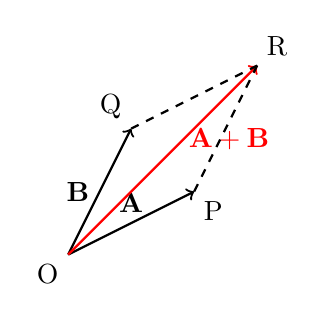
\begin{tikzpicture}[scale=0.8]
        % ... (código de la figura del paralelogramo) ...
     
  \draw[thick,->] (0,0) -- (2,1) node[midway, above] {$\mathbf{A}$}; % Vector A
  \draw[thick,->] (0,0) -- (1,2) node[midway, left] {$\mathbf{B}$}; % Vector B

  \draw[thick,->,red] (0,0) -- (3,3) node[midway, above right, xshift=2mm ] {$\mathbf{A} + \mathbf{B}$}; % Vector A + B
  \draw[thick,dashed] (2,1) -- (3,3); % Lado del paralelogramo
  \draw[thick,dashed] (1,2) -- (3,3); % Lado del paralelogramo

  % Puedes agregar etiquetas para los vértices si lo deseas
   \node[below left] at (0,0) {O};
   \node[below right] at (2,1) {P};
   \node[above left] at (1,2) {Q};
   \node[above right] at (3,3) {R};

    \end{tikzpicture}
    \caption{Suma de vectores mediante el método del paralelogramo.}
    \label{fig:paralelogramo}
    \end{wrapfigure}
  
\textbf{Método del paralelogramo:} Se dibujan los vectores $\mathbf{A}$ y $\mathbf{B}$ con su origen en el mismo punto. Luego, se construye un \\paralelogramo con $\mathbf{A}$ y $\mathbf{B}$ como lados adyacentes. La diagonal del paralelogramo que parte del origen común de $\mathbf{A}$ y $\mathbf{B}$ representa la suma $\mathbf{A} + \mathbf{B}$. 

% Continúa con el resto del texto...

\textbf{Método analítico:} Para sumar vectores analíticamente, se suman las componentes correspondientes de cada vector. Si $\mathbf{A} = (A_x, A_y, A_z)$ y $\mathbf{B} = (B_x, B_y, B_z)$, entonces $\mathbf{A} + \mathbf{B} = (A_x + B_x, A_y + B_y, A_z + B_z)$.
\newpage

\begin{minipage}{0.9\textwidth}
  \textbf{Resta de vectores:}
\begin{itemize}
\item \textbf{Definición:} La resta de dos vectores $\mathbf{A}$ y $\mathbf{B}$ se define como la suma del vector $\mathbf{A}$ con el opuesto del vector $\mathbf{B}$, es decir, $\mathbf{A} - \mathbf{B} = \mathbf{A} + (-\mathbf{B})$.
\item \textbf{Método gráfico:} Para restar dos vectores $\mathbf{A}$ y $\mathbf{B}$ gráficamente, se dibuja el vector $\mathbf{A}$ y el vector $-\mathbf{B}$ (que tiene la misma magnitud que $\mathbf{B}$ pero sentido opuesto). Luego, se suman los vectores $\mathbf{A}$ y $-\mathbf{B}$ utilizando el método del paralelogramo.
\item \textbf{Método analítico:} Para restar vectores analíticamente, se restan las componentes correspondientes de cada vector. Si $\mathbf{A} = (A_x, A_y, A_z)$ y $\mathbf{B} = (B_x, B_y, B_z)$, entonces $\mathbf{A} - \mathbf{B} = (A_x - B_x, A_y - B_y, A_z - B_z)$.
\end{itemize}
  
\end{minipage}

\textbf{Propiedades de la suma y resta de vectores:}

\begin{itemize}
\item \textbf{Conmutatividad:} La suma de vectores es conmutativa: $\mathbf{A} + \mathbf{B} = \mathbf{B} + \mathbf{A}$.
\item \textbf{Asociatividad:} La suma de vectores es asociativa: $(\mathbf{A} + \mathbf{B}) + \mathbf{C} = \mathbf{A} + (\mathbf{B} + \mathbf{C})$.
\item \textbf{Existencia del vector cero:} Existe un vector cero, denotado como $\mathbf{0}$, que cumple que $\mathbf{A} + \mathbf{0} = \mathbf{A}$ para cualquier vector $\mathbf{A}$.
\item \textbf{Existencia del vector opuesto:} Para cada vector $\mathbf{A}$ existe un vector opuesto $-\mathbf{A}$, tal que $\mathbf{A} + (-\mathbf{A}) = \mathbf{0}$.
\end{itemize}

\textbf{Aplicaciones:} La suma y resta de vectores tienen numerosas aplicaciones en física e ingeniería, como el cálculo de fuerzas resultantes, velocidades resultantes, análisis de circuitos eléctricos (fasores), etc.

\subsection{Multiplicación de un vector por un escalar}

\textbf{Introducción:}

En el álgebra vectorial, no solo podemos sumar y restar vectores, sino que también podemos multiplicarlos por escalares (números reales). Esta operación, aunque sencilla en apariencia, tiene un gran impacto en la forma en que representamos y manipulamos magnitudes físicas. Imaginemos, por ejemplo, que queremos duplicar la fuerza que se aplica sobre un objeto, o que necesitamos invertir el sentido del campo eléctrico en una región del espacio. ¿Cómo podemos lograr esto? La respuesta está en la multiplicación de un vector por un escalar.

Esta operación nos da un "control" similar al que tenemos con los filtros de Instagram. Así como podemos aumentar el brillo o la saturación de una foto, al multiplicar un vector por un escalar podemos modificar su magnitud y dirección, creando nuevas posibilidades para describir el mundo que nos rodea.
\newpage
\textbf{Definición:}

Al multiplicar un vector $\mathbf{A}$ por un escalar $k$, se obtiene un nuevo vector $k\mathbf{A}$ cuya magnitud es $|k|$ veces la magnitud de $\mathbf{A}$, y cuya dirección es la misma que la de $\mathbf{A}$ si $k$ es positivo, o la opuesta si $k$ es negativo.

\begin{figure}[H]
\centering
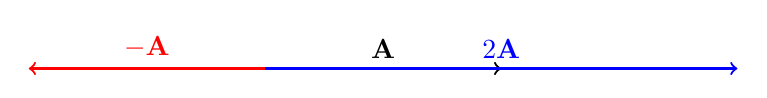
\begin{tikzpicture}[scale=1.5]

  \draw[thick,->] (0,0) -- (2,0) node[midway, above] {$\mathbf{A}$}; % Vector A
  \draw[thick,->,blue] (0,0) -- (4,0) node[midway, above] {$2\mathbf{A}$}; % Vector 2A
  \draw[thick,->,red] (0,0) -- (-2,0) node[midway, above] {$-\mathbf{A}$}; % Vector -A

\end{tikzpicture}
\caption{Multiplicación del vector $\mathbf{A}$ por los escalares 2 y -1.}
\label{fig:multiplicacion_escalar}
\end{figure}

Ejemplo:

Si $\mathbf{A}$ es un vector de magnitud 3 unidades que apunta hacia la derecha, y $k = 2$, entonces $2\mathbf{A}$ será un vector de magnitud 6 unidades que también apunta hacia la derecha. Si $k = -1$, entonces $-\mathbf{A}$ será un vector de magnitud 3 unidades que apunta hacia la izquierda.

\textbf{En resumen:}

\begin{itemize}
\item[\textbullet] La multiplicación por un escalar positivo estira o comprime el vector, manteniendo su dirección.
\item[\textbullet] La multiplicación por un escalar negativo estira o comprime el vector e invierte su dirección.
\end{itemize}

\textbf{Propiedades de la multiplicación por un escalar:}

La multiplicación de un vector por un escalar cumple con las siguientes propiedades:

\begin{itemize}
\item[\textbullet] \textbf{Distributiva respecto a la suma de vectores:} $k (\mathbf{A} + \mathbf{B}) = k\mathbf{A} + k\mathbf{B}$
\item[\textbullet] \textbf{Distributiva respecto a la suma de escalares:} $(k + l)\mathbf{A} = k\mathbf{A} + l\mathbf{A}$
\item[\textbullet] \textbf{Asociativa:} $(k l)\mathbf{A} = k(l\mathbf{A})$
\item[\textbullet] \textbf{Multiplicación por 1:} $1\mathbf{A} = \mathbf{A}$
\end{itemize}

Estas propiedades son similares a las propiedades de la multiplicación de números reales, y nos permiten manipular expresiones con vectores y escalares de forma flexible.

\subsection{Producto de vectores}

\textbf{Introducción:}

Además de la suma, la resta y la multiplicación por un escalar, existen otras operaciones que podemos realizar con vectores. En particular, el producto escalar y el producto vectorial son dos operaciones que combinan dos vectores para producir un nuevo objeto (un escalar o un vector, respectivamente).

\subsubsection{Producto escalar o producto punto}

\textbf{Definición:} El producto escalar de dos vectores $\mathbf{A}$ y $\mathbf{B}$, denotado por $\mathbf{A} \cdot \mathbf{B}$, se define como el producto de sus magnitudes y el coseno del ángulo entre ellos:

%$\mathbf{A} \cdot \mathbf{B} = |\mathbf{A}||\mathbf{B}| \cos \theta$
\begin{empheq}[box=\fbox]{align*}
\mathbf{A} \cdot \mathbf{B} &\equiv |\mathbf{A}||\mathbf{B}| \cos \theta
\end{empheq}

donde $|\mathbf{A}|$ y $|\mathbf{B}|$ son las magnitudes de los vectores $\mathbf{A}$ y $\mathbf{B}$ respectivamente, y $\theta$ es el ángulo entre ellos.

\textbf{Interpretación geométrica:} El producto escalar se puede interpretar geométricamente como el producto de la magnitud de la proyección de $\mathbf{A}$ sobre $\mathbf{B}$ por la magnitud de $\mathbf{B}$.

$\mathbf{A} \cdot \mathbf{B} = (A \cos \theta) |\mathbf{B}| = |\mathbf{A}| (B \cos \theta)$

\begin{figure}[H]
\centering
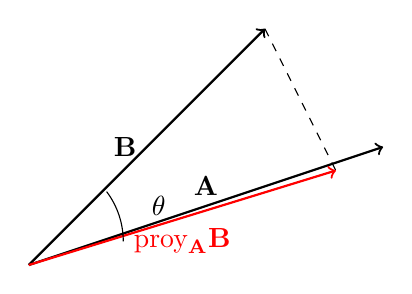
\begin{tikzpicture}[scale=1.5]

  \draw[thick,->] (0,0) -- (3,1) node[midway, above] {$\mathbf{A}$}; % Vector A
  \draw[thick,->] (0,0) -- (2,2) node[midway, left] {$\mathbf{B}$}; % Vector B

  \draw[dashed] (2,2) -- (2.6,0.8); % Línea de proyección
  \draw[thick,->,red] (0,0) -- (2.6,0.8) node[midway, below] {$\text{proy}_{\mathbf{A}} \mathbf{B}$}; % Proyección de B sobre A

  % Ángulo entre los vectores
  \draw[thin] (0.8,0.2) arc (0:37:0.7); % Coordenadas modificadas
  \node at (1.1,0.5) {$\theta$}; % Coordenadas modificadas

\end{tikzpicture}
\caption{Proyección del vector $\mathbf{B}$ sobre el vector $\mathbf{A}$.}
\label{fig:proyeccion_vectorial_B_sobre_A}
\end{figure}

\textbf{Propiedades:} El producto escalar tiene las siguientes propiedades:

\begin{itemize}
\item[\textbullet] \textbf{Conmutatividad:} $\mathbf{A} \cdot \mathbf{B} = \mathbf{B} \cdot \mathbf{A}$
\item[\textbullet] \textbf{Distributividad:} $\mathbf{A} \cdot (\mathbf{B} + \mathbf{C}) = \mathbf{A} \cdot \mathbf{B} + \mathbf{A} \cdot \mathbf{C}$
\item[\textbullet] \textbf{Asociatividad con un escalar:} $(k\mathbf{A}) \cdot \mathbf{B} = k(\mathbf{A} \cdot \mathbf{B}) = \mathbf{A} \cdot (k\mathbf{B})$
\item[\textbullet] \textbf{Producto de un vector por sí mismo:} $\mathbf{A} \cdot \mathbf{A} = |\mathbf{A}|^2$
\end{itemize}

\textbf{Expresión en coordenadas cartesianas:} Si $\mathbf{A} = (A_x, A_y, A_z)$ y $\mathbf{B} = (B_x, B_y, B_z)$, entonces:

$\mathbf{A} \cdot \mathbf{B} = A_xB_x + A_yB_y + A_zB_z$

\textbf{Aplicaciones:} El producto escalar tiene numerosas aplicaciones en física e ingeniería, tales como:

\begin{itemize}
\item[\textbullet] Calcular el trabajo realizado por una fuerza.
\item[\textbullet] Determinar el ángulo entre dos vectores.
\item[\textbullet] Calcular la componente de un vector en una dirección dada.
\item[\textbullet] Verificar si dos vectores son ortogonales (perpendiculares).
\end{itemize}

\subsubsection{Producto Vectorial o Producto Cruz}

\textbf{Definición:} El producto vectorial de dos vectores $\mathbf{A}$ y $\mathbf{B}$, denotado por $\mathbf{A} \times \mathbf{B}$, es un nuevo vector $\mathbf{C}$ cuya definición es: “el vector cuya magnitud es el valor absoluto del producto de las magnitudes de los dos vectores por el seno del
ángulo menor entre los dos vectores mientras que la dirección del vector es perpendicular al plano en el que se encuentran los dos vectores”
\begin{empheq}[box=\fbox]{align*}
|\mathbf{C}| = |\mathbf{A} \times \mathbf{B}| &\equiv |\mathbf{A}| |\mathbf{B}| \sin \theta
\end{empheq}
\begin{itemize}
\item[\textbullet]Magnitud: La magnitud de $\mathbf{C}$ es igual al producto de las magnitudes de $\mathbf{A}$ y $\mathbf{B}$ por el seno del ángulo $\theta$ entre ellos:
  %$|\mathbf{C}| = |\mathbf{A} \times \mathbf{B}| = |\mathbf{A}| |\mathbf{B}| \sin \theta$

\item[\textbullet] Dirección $\mathbf{C}$ es perpendicular al plano que contiene a los vectores $\mathbf{A}$ y $\mathbf{B}$.
\item[\textbullet]Sentido: El sentido de $\mathbf{C}$ se determina por la regla de la mano derecha: Si se coloca la mano derecha de manera que los dedos apunten en la dirección del vector $\mathbf{A}$ y se curvan hacia el vector $\mathbf{B}$ a través del ángulo $\theta$, entonces el pulgar apuntará en la dirección de $\mathbf{C}$. El ángulo $\theta$ es el menor de los ángulos que se pueden formar entre ambos vectores.
\item[\textbullet]Interpretación geométrica: La magnitud del producto vectorial $|\mathbf{A} \times \mathbf{B}|$ es igual al área del paralelogramo formado por los vectores $\mathbf{A}$ y $\mathbf{B}$.
\end{itemize}

\textbf{Propiedades:} El producto vectorial tiene las siguientes propiedades:
\begin{itemize}
    \item[\textbullet] Anticonmutatividad: $\mathbf{A} \times \mathbf{B} = - (\mathbf{B} \times \mathbf{A})$
    \item[\textbullet] Distributividad: $\mathbf{A} \times (\mathbf{B} + \mathbf{C}) = \mathbf{A} \times \mathbf{B} + \mathbf{A} \times \mathbf{C}$
    \item[\textbullet] Asociatividad con un escalar: $(k \mathbf{A}) \times \mathbf{B} = k (\mathbf{A} \times \mathbf{B}) = \mathbf{A} \times (k \mathbf{B})$
    \item[\textbullet] Producto vectorial por sí mismo: $\mathbf{A} \times \mathbf{A} = \mathbf{0}$
\end{itemize}


\textbf{Expresión en coordenadas cartesianas:} Si $\mathbf{A} = (A_x, A_y, A_z)$ y $\mathbf{B} = (B_x, B_y, B_z)$, entonces el producto vectorial $\mathbf{A} \times \mathbf{B}$ se puede calcular mediante el siguiente determinante:

$\mathbf{A} \times \mathbf{B} =
\begin{vmatrix}
\mathbf{i} & \mathbf{j} & \mathbf{k} \\
A_x & A_y & A_z \\
B_x & B_y & B_z
\end{vmatrix}$
donde $\mathbf{i}$, $\mathbf{j}$ y $\mathbf{k}$ son los vectores unitarios en las direcciones $x$, $y$ y $z$ respectivamente.

\textbf{Aplicaciones:} El producto vectorial tiene numerosas aplicaciones en física e ingeniería, tales como:
\begin{itemize}
    \item [\textbullet] Calcular el momento de una fuerza.
    \item[\textbullet] Calcular el flujo magnético a través de una superficie
    \item[\textbullet] Describir la fuerza magnética sobre una carga en movimiento 
\end{itemize}

\begin{figure}[H]
\centering
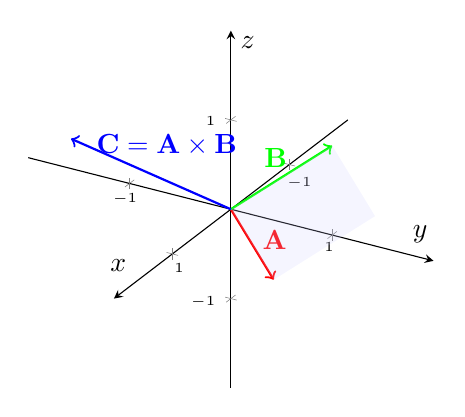
\begin{tikzpicture}
\begin{axis}[
    view={120}{30}, % Ajusta la vista 3D
    axis lines=center,
    xlabel=$x$,
    ylabel=$y$,
    zlabel=$z$,
    xmin=-2, xmax=2,
    ymin=-2, ymax=2,
    zmin=-2, zmax=2,
    xtick={-1,0,1}, 
    ytick={-1,0,1}, 
    ztick={-1,0,1}, % Ajusta las marcas de los ejes
    xticklabel style={font=\tiny},
    yticklabel style={font=\tiny},
    zticklabel style={font=\tiny},
    width=0.8\textwidth,  % Ancho de la figura
    height=0.8\textwidth, % Altura de la figura (ajustada proporcionalmente)
]

% Define los vectores A y B
\coordinate (A) at (1,1,0);
\coordinate (B) at (0,1,1);

% Dibuja los vectores A y B
\draw[thick,->,red] (axis cs:0,0,0) -- (axis cs:1,1,0) node[midway, above right, yshift=-2mm] {$\mathbf{A}$};
\draw[thick,->,green] (axis cs:0,0,0) -- (axis cs:0,1,1) node[midway, above left, xshift=2mm] {$\mathbf{B}$};

% Calcula el producto vectorial C = A x B
\coordinate (C) at (1,-1,1);

% Dibuja el vector C
\draw[thick,->,blue] (axis cs:0,0,0) -- (axis cs:1,-1,1) node[midway, above, xshift=2mm, yshift=1mm] {$\mathbf{C} = \mathbf{A} \times \mathbf{B}$};

% Dibuja el plano formado por A y B con sombreado
\fill[opacity=0.2, blue!20] (axis cs:0,0,0) -- (axis cs:1,1,0) -- (axis cs:1,2,1) -- (axis cs:0,1,1) -- cycle;

\end{axis}
\end{tikzpicture}
\caption{Producto vectorial de dos vectores $\mathbf{A}$ y $\mathbf{B}$. El vector resultante $\mathbf{C}$ es perpendicular al plano formado por $\mathbf{A}$ y $\mathbf{B}$.}
\label{fig:producto_vectorial_sin_proyecciones}
\end{figure}


\subsection{Definición de campos}

\textbf{Introducción:}

Un campo es una región del espacio donde se define una magnitud física en cada punto. Esta magnitud puede ser escalar o vectorial, lo que da lugar a dos tipos de campos: campos escalares y campos vectoriales.

Esta idea es similar a la de las funciones de varias variables que estudiaron en Análisis Matemático II. Así como una función $f(x, y, z)$ asigna un valor a cada punto $(x, y, z)$ en el espacio, un campo también asigna una magnitud (escalar o vectorial) a cada punto.

\subsubsection{Campos escalares:}

Un campo escalar es aquel en el que a cada punto del espacio se le asigna un valor numérico (un escalar). Podemos representarlo matemáticamente como una función escalar de tres variables: $f(x, y, z)$ donde $f$ es el valor del campo escalar en el punto $(x, y, z)$.

\textbf{Ejemplos:}
\begin{itemize}
    \item [\textbullet]Temperatura en una habitación: $T(x, y, z)$
    \item [\textbullet]Presión atmosférica: $P(x, y, z)$
    \item [\textbullet]Potencial eléctrico: $V(x, y, z)$
    \item [\textbullet]Densidad de carga: $\rho(x, y, z)$
\end{itemize}

\subsubsection{Campos vectoriales:}

Un campo vectorial es aquel en el que a cada punto del espacio se le asigna un vector. Podemos representarlo matemáticamente como una función vectorial:

$\mathbf{F}(x, y, z) = F_x(x, y, z) \mathbf{\hat{a}}_x + F_y(x, y, z) \mathbf{\hat{a}}_y + F_z(x, y, z) \mathbf{\hat{a}}_z$ donde $\mathbf{F}$ es el vector del campo en el punto $(x, y, z)$, y $F_x$, $F_y$, $F_z$ son sus componentes escalares en las direcciones de los vectores unitarios $\mathbf{\hat{a}}_x$, $\mathbf{\hat{a}}_y$ y $\mathbf{\hat{a}}_z$.

\textbf{Ejemplos:}
\begin{itemize}
    \item [\textbullet]Campo gravitatorio: $\mathbf{g}(x, y, z)$
    \item [\textbullet]Campo eléctrico: $\mathbf{E}(x, y, z)$
    \item [\textbullet]Campo magnético: $\mathbf{H}(x, y, z)$ (o $\mathbf{B}(x, y, z)$)
    \item [\textbullet]Velocidad del viento: $\mathbf{v}(x, y, z)$
\end{itemize}

\textbf{Representación gráfica de campos escalares}

\textbf{Introducción:}

Para visualizar un campo escalar, utilizamos mapas de isolíneas o curvas de nivel. Estas son curvas que conectan puntos con el mismo valor del campo. Imagina un mapa topográfico, donde las curvas de nivel representan puntos con la misma altitud. De manera similar, en un mapa de isolíneas de un campo escalar, las curvas conectan puntos con el mismo valor del campo.
    
\textbf{Construcción de un mapa de isolíneas:}
\begin{wrapfigure}{r}{0.4\textwidth} % "r" para colocar la figura a la derecha, 0.4\textwidth para el ancho
    \centering
    \begin{tikzpicture}
    \begin{axis}[
        view={0}{90}, % Vista 2D desde arriba
        axis equal image, % Misma escala en ambos ejes
        xlabel=$x$,
        ylabel=$y$,
        xmin=-2, xmax=2,
        ymin=-2, ymax=2,
        xtick=\empty, ytick=\empty, % Oculta las marcas de los ejes
        colorbar, % Muestra la barra de colores
        colormap/cool, % Mapa de colores
    ]

    \addplot3[
        contour gnuplot={levels={-2,-1,-0.5,0,0.5,1,2}, labels=false}, % Define los niveles de las isolíneas
        domain=-2:2,
        domain y=-2:2,
        samples=25, % Ajusta la densidad de la malla
    ]
   {1/((x-1)^2+y^2)^(1/2) - 1/((x+1)^2+y^2)^(1/2)}; % Función del potencial eléctrico

    \end{axis}
    \end{tikzpicture}
    $\frac{1}{\sqrt{(x-1)^2 + y^2}} - \frac{1}{\sqrt{(x+1)^2 + y^2}}$; % Función del potencial eléctrico
    \caption{Potencial eléctrico visto desde arriba.}
\end{wrapfigure}

Para construir un mapa de isolíneas, seguimos estos pasos:

\begin{enumerate}
\item Elegimos un conjunto de valores representativos del campo escalar.
\item Para cada valor, identificamos los puntos en el espacio que tienen ese valor.
\item Unimos esos puntos mediante curvas suaves, que son las isolíneas.
\end{enumerate}

\textbf{Características de las isolíneas:}

Las isolíneas tienen características importantes que nos ayudan a interpretar el campo escalar:

\begin{itemize}
\item[\textbullet] Las isolíneas nunca se cruzan entre sí, ya que un punto en el espacio no puede tener dos valores diferentes del campo escalar.
\item[\textbullet] La densidad de las isolíneas indica la magnitud del gradiente del campo escalar: cuanto más juntas estén las isolíneas, mayor es el gradiente (o variación) del campo en esa región. Veremos el concepto de gradiente en detalle en el próximo módulo.
\item[\textbullet] Las isolíneas cerradas indican máximos o mínimos locales del campo escalar.
\end{itemize}

\textbf{Ejemplos:}

Veamos algunos ejemplos de campos escalares y sus mapas de isolíneas:

\begin{itemize}
\item[\textbullet] \textbf{Temperatura en una habitación:} Las isolíneas conectarían puntos con la misma temperatura. Podríamos observar zonas más calientes y zonas más frías en la habitación.
\item[\textbullet] \textbf{Presión atmosférica:} En un mapa meteorológico, las isolíneas de presión (isobaras) conectan puntos con la misma presión atmosférica. Estas líneas nos ayudan a identificar zonas de alta y baja presión, que están relacionadas con los fenómenos climáticos.
\item[\textbullet] \textbf{Potencial eléctrico:} Las isolíneas de potencial eléctrico (equipotenciales) conectan puntos con el mismo potencial. Estas líneas nos ayudan a visualizar la distribución del potencial eléctrico en una región con cargas.
\end{itemize}

\textbf{Herramientas para la visualización:}

Para crear mapas de isolíneas, podemos utilizar diferentes herramientas:

\begin{itemize}
\item[\textbullet] \textbf{Lenguajes de programación:} Phyton, MATLAB.
\item[\textbullet] \textbf{Software de graficación:} Gnuplot.
\item[\textbullet] \textbf{Herramientas online:} Existen varias herramientas online que permiten crear mapas de isolíneas de forma interactiva.
\end{itemize}

%campo eléctrico vectorial gráfica 3D
  
\begin{figure}[H] % Agrega el entorno figure con la opción [H]
\centering
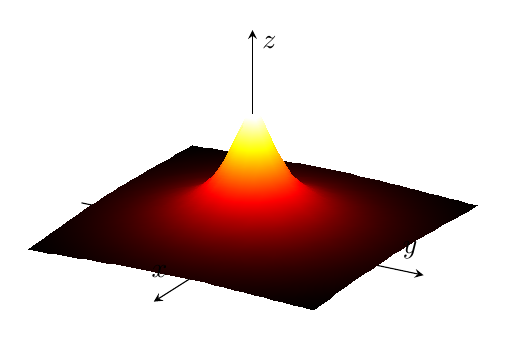
\begin{tikzpicture}
\begin{axis}[
    view={120}{30}, % Ajusta la vista 3D
    axis lines=center,
    xlabel=$x$,
    ylabel=$y$,
    zlabel=$z$,
    xmin=-3, xmax=3,
    ymin=-3, ymax=3,
    zmin=-1, zmax=5,
    xtick=\empty, ytick=\empty, ztick=\empty, % Oculta las marcas de los ejes
    colormap/hot2, % Mapa de colores
]

\addplot3[
    surf,
    shader=interp, % Interpolación de colores
    domain=-2.5:2.5,
    domain y=-2.5:2.5,
    samples=30, % Ajusta la densidad de la malla
    z buffer=sort,
]
{1/((x^2+y^2+0.1)^(1/2))}; % Función del potencial eléctrico

\end{axis}
\end{tikzpicture}
$\frac{1}{\sqrt{x^2 + y^2 + 0.1}}$ Función del potencial eléctrico
\caption{Potencial eléctrico generado por una carga puntual.}
\end{figure}
 



\newpage
\subsection{Sistemas de coordenadas}

\textbf{Introducción:}

\subsection{Sistemas de coordenadas}

En el estudio del electromagnetismo, es fundamental poder describir la posición de cargas, corrientes y campos en el espacio. Para ello, utilizamos sistemas de coordenadas, que son conjuntos de reglas que nos permiten especificar la ubicación de un punto. En esta sección, estudiaremos los tres sistemas de coordenadas más utilizados en electromagnetismo: cartesiano, cilíndrico y esférico.

Una característica importante de estos sistemas es que son \textbf{ortogonales}: los vectores unitarios que definen las direcciones de los ejes son perpendiculares entre sí en cada punto del espacio. Esto significa que, al representar un punto en cualquiera de estos sistemas, lo hacemos en referencia a vectores unitarios que forman ángulos rectos entre sí. 

Es importante destacar que, aunque algunos vectores unitarios representan desplazamientos lineales (como $\mathbf{\hat{a}}_x$, $\mathbf{\hat{a}}_y$, $\mathbf{\hat{a}}_z$ en coordenadas cartesianas o  $\mathbf{\hat{a}}_\rho$ en coordenadas cilíndricas) y otros representan desplazamientos angulares (como $\mathbf{\hat{a}}_\phi$ en coordenadas cilíndricas o $\mathbf{\hat{a}}_\theta$ y $\mathbf{\hat{a}}_\phi$ en coordenadas esféricas), la ortogonalidad se mantiene. Los vectores unitarios, ya sean lineales o angulares, siempre son perpendiculares entre sí en cada punto del espacio.

La ortogonalidad de los sistemas de coordenadas facilita la descripción de fenómenos físicos y la resolución de problemas en electromagnetismo. Por ejemplo, al calcular la fuerza entre dos cargas, podemos descomponerla en sus componentes a lo largo de los ejes ortogonales, lo que simplifica el análisis.


\subsubsection{Sistema de coordenadas cartesianas:}

El sistema cartesiano es el más familiar. Utiliza tres ejes perpendiculares entre sí, que se suelen denotar como $x$, $y$ y $z$. La posición de un punto se define mediante sus coordenadas $(x, y, z)$, que representan las distancias del punto a cada uno de los planos formados por los otros dos ejes.

Los vectores unitarios en este sistema se denotan como $\mathbf{\hat{a}}_x$, $\mathbf{\hat{a}}_y$ y $\mathbf{\hat{a}}_z$, y apuntan en la dirección positiva de los ejes $x$, $y$ y $z$ respectivamente.

Las coordenadas cartesianas son especialmente útiles en problemas donde la geometría se alinea con los ejes cartesianos, como el cálculo del campo eléctrico o del potencial eléctrico debido a la distribución de cargas puntuales o lineales a lo largo de un alambre finito cargado.
 
 
\tdplotsetmaincoords{70}{110}  % Nuevos ángulos de visión
\begin{tikzpicture}[tdplot_main_coords, scale=1.5]
  \draw[thick,->] (0,0,0) -- (4,0,0) node[anchor=north east]{$x$};
  \draw[thick,->] (0,0,0) -- (0,4,0) node[anchor=north west]{$y$};
  \draw[thick,->] (0,0,0) -- (0,0,4) node[anchor=south]{$z$};

  %\draw[thick,->,blue] (0,0,0) -- (2,2,2) node[midway,above]; 

  % Proyecciones como caja en líneas de trazos
  \draw[dashed] (2,0,0) -- (2,2,0) -- (0,2,0);
  \draw[dashed] (2,2,0) -- (2,2,2) -- (0,2,2) -- (0,0,2);
  \draw[dashed] (0,0,2) -- (2,0,2) -- (2,2,2);
  \draw[dashed] (2,0,0) -- (2,0,2);
  \draw[dashed] (0,2,0) -- (0,2,2);
  \node[anchor=south west, above] at (2,2,2){\textcolor{blue}{P(x,y,z)}};
  \node[anchor=north, above left] at (2,0,0) {$x$};
  \node[anchor=east, above left] at (0,2,0) {$y$};
  \node[anchor=west, above right] at (0,0,2) {$z$};
\end{tikzpicture}

\end{document}






